\documentclass{beamer}

\usetheme{Madrid}
\usecolortheme{default}
\usepackage[utf8]{inputenc}
\usepackage{graphicx}
\usepackage{booktabs}
\usepackage{hyperref}

\title[Refining ISN to V3]{Refining the Sunspot Number Series to ISN~V3:\\ Challenges and Benefits for the Space Climate Community}
\author{FARSuN Project (Findability and Accessibility of historical Raw Sunspot Numbers)}
\institute{Royal Observatory of Belgium (ROB) / SILSO and collaborators}
\date{ESWW 2025}

\begin{document}

% --- Title ---
\begin{frame}
  \titlepage
\end{frame}

% --- Abstract ---
\begin{frame}{Abstract}
The International Sunspot Number (ISN) series, a cornerstone for space climate studies, still exhibits scale discrepancies despite recent recalibrations.  

\medskip
The FARSuN project addresses this by systematically gathering, digitizing, and standardizing raw sunspot data from 1607--1980.  
\medskip

\textbf{Goals:}
\begin{itemize}
  \item Comprehensive reconstruction, not just recalibration
  \item Homogeneous metadata and uncertainties
  \item Citizen science engagement
  \item Deliver ISN V3 + hemispheric numbers
\end{itemize}
\end{frame}

% --- Problem ---
\begin{frame}{The Problem with ISN}
\begin{itemize}
  \item Longest record of solar variability
  \item But inhomogeneities remain: e.g.\ “Waldmeier jump” around 1947
  \item Past fixes = recalibration $\rightarrow$ still limited
\end{itemize}
\end{frame}

% --- Reconstruction vs Recalibration ---
\begin{frame}{Reconstruction vs.\ Recalibration}
\begin{columns}
\column{0.48\textwidth}
\textbf{Recalibration}
\begin{itemize}
  \item Adjusts existing index
  \item May propagate hidden biases
\end{itemize}

\column{0.48\textwidth}
\textbf{Reconstruction}
\begin{itemize}
  \item Returns to raw observations
  \item Systematic metadata + QC
  \item More robust and transparent
\end{itemize}
\end{columns}
\end{frame}

% --- FARSuN Approach ---
\begin{frame}{FARSuN’s Four-Axis Methodology}
\begin{enumerate}
  \item Gather Sources – archives, manuscripts, tables
  \item Process Data – digitize, OCR/HWR (Transkribus)
  \item Validate \& Standardize – homogeneous metadata, QC/QA
  \item Disseminate – FAIR principles, VO-ready access
\end{enumerate}
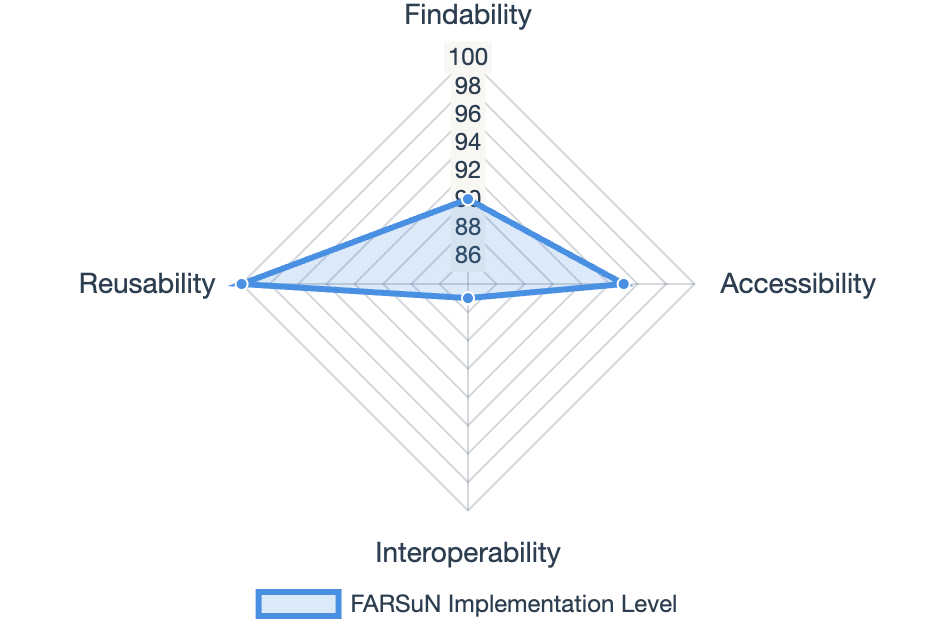
\includegraphics[width=0.6\linewidth]{./figures/fair_radar.png}
\end{frame}

% --- Key Datasets ---
\begin{frame}{Key Datasets}
\begin{itemize}
  \item Zürich Tables (1945--1979): $\sim$95\% digitized
  \item \emph{Mittheilungen} (1610--1918): integrated
  \item Gruithuisen: early 19th c., Kurrent script
  \item C.H. Adams: 19--20c, drawings
  \item Stark, Rost: tabular, metadata harmonization
\end{itemize}
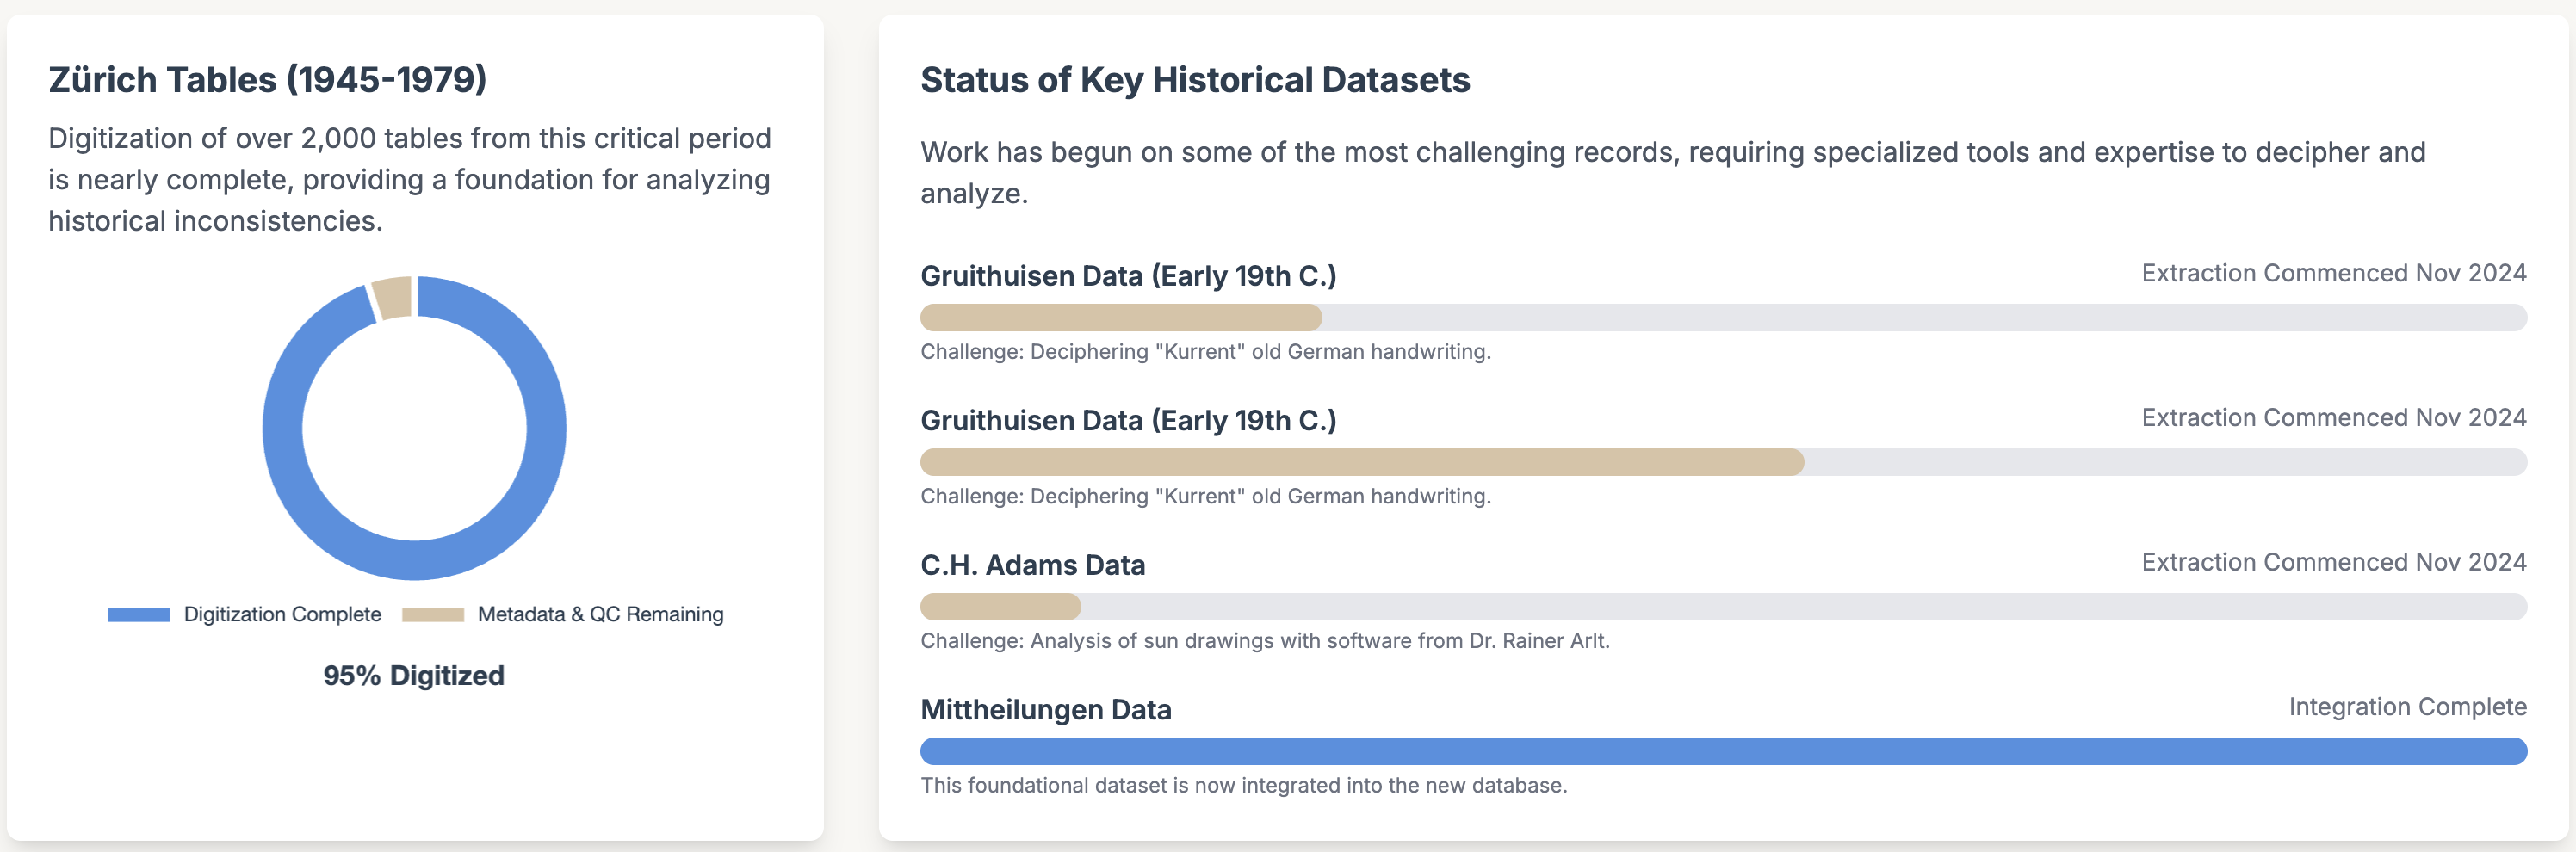
\includegraphics[width=0.7\linewidth]{./figures/dataset_progress.png}
\end{frame}

% --- Observer Timeline ---
\begin{frame}{Observer Timeline}
\centering
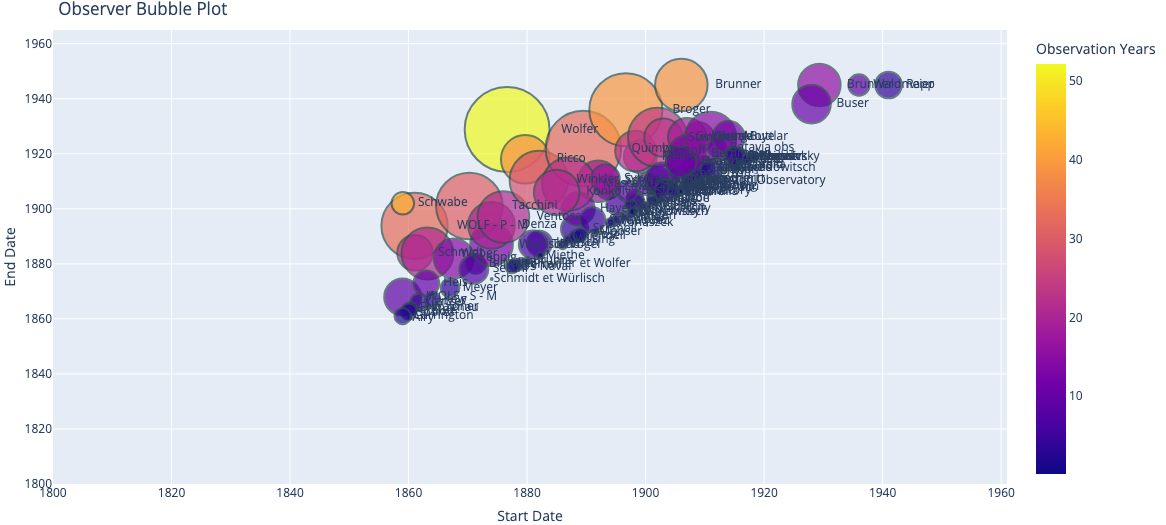
\includegraphics[width=0.9\linewidth]{./figures/observers_bubble.png}

{\scriptsize Bubble size = total observations; color = years}
\end{frame}

% --- Comparison ---
\begin{frame}{From Raw Data to ISN V3}
\begin{enumerate}
  \item Curate daily group/spot counts
  \item Cross-calibrate observers
  \item Aggregate monthly/yearly
  \item Compare to SN V2
\end{enumerate}
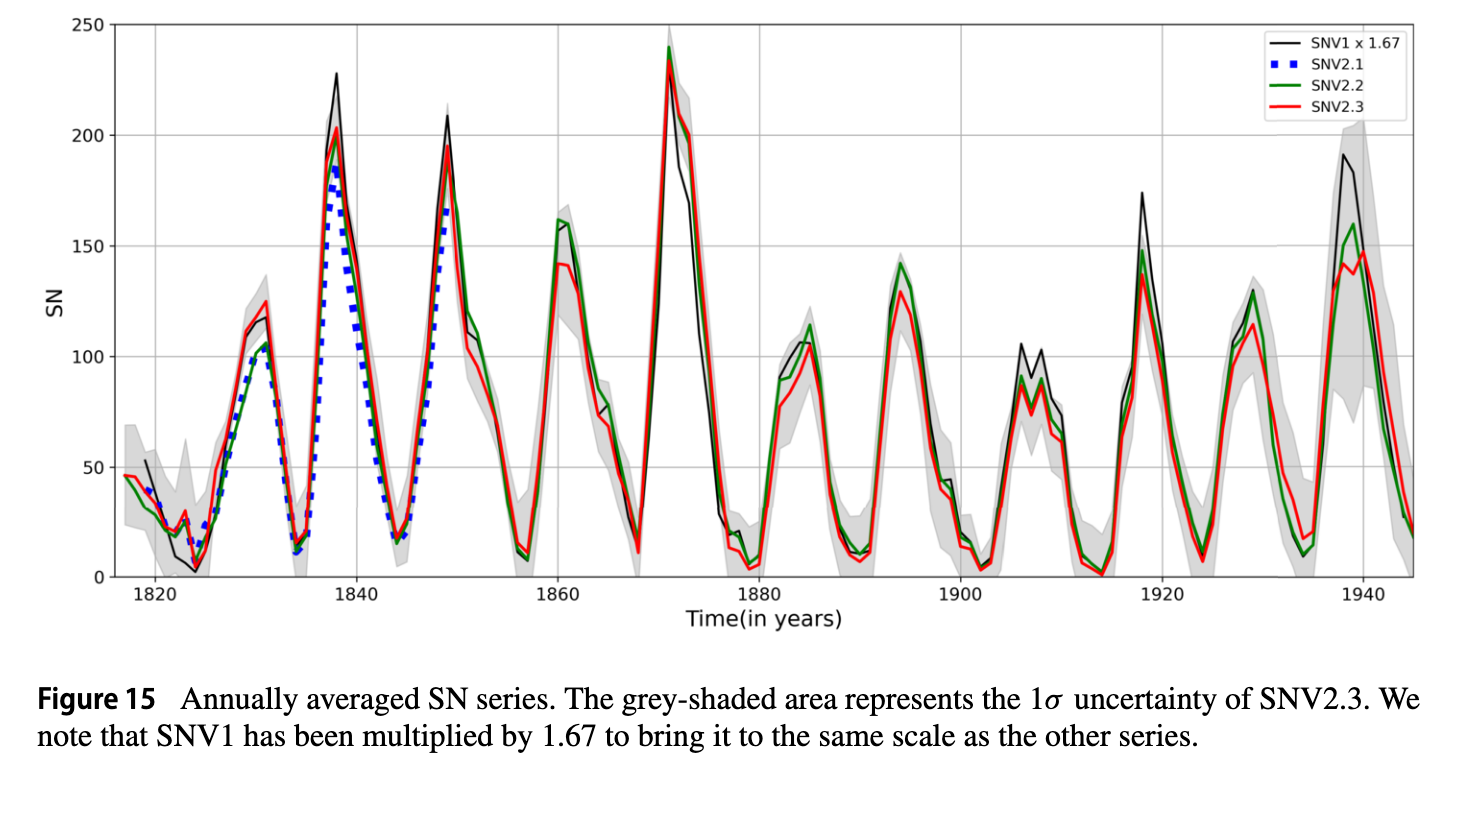
\includegraphics[width=0.75\linewidth]{./figures/comparison_panel.png}
\end{frame}

% --- Challenges ---
\begin{frame}{Challenges}
\begin{itemize}
  \item Handwriting: old German \emph{Kurrent}
  \item Heterogeneous formats (drawings, tables, text)
  \item Observer-dependent biases
  \item Provenance + uncertainty propagation
\end{itemize}
\end{frame}

% --- Impact ---
\begin{frame}{Impact for Space Climate}
\begin{itemize}
  \item More accurate cycle predictions
  \item Long-term solar variability studies
  \item Space weather baselines
  \item Improved climate model inputs
\end{itemize}
\end{frame}

% --- Outlook ---
\begin{frame}{Outlook}
\begin{itemize}
  \item Citizen science portal (public data recovery)
  \item Consolidated ISN V3 + hemispheric series
  \item FAIR, open-access dissemination
  \item Collaboration open to community
\end{itemize}
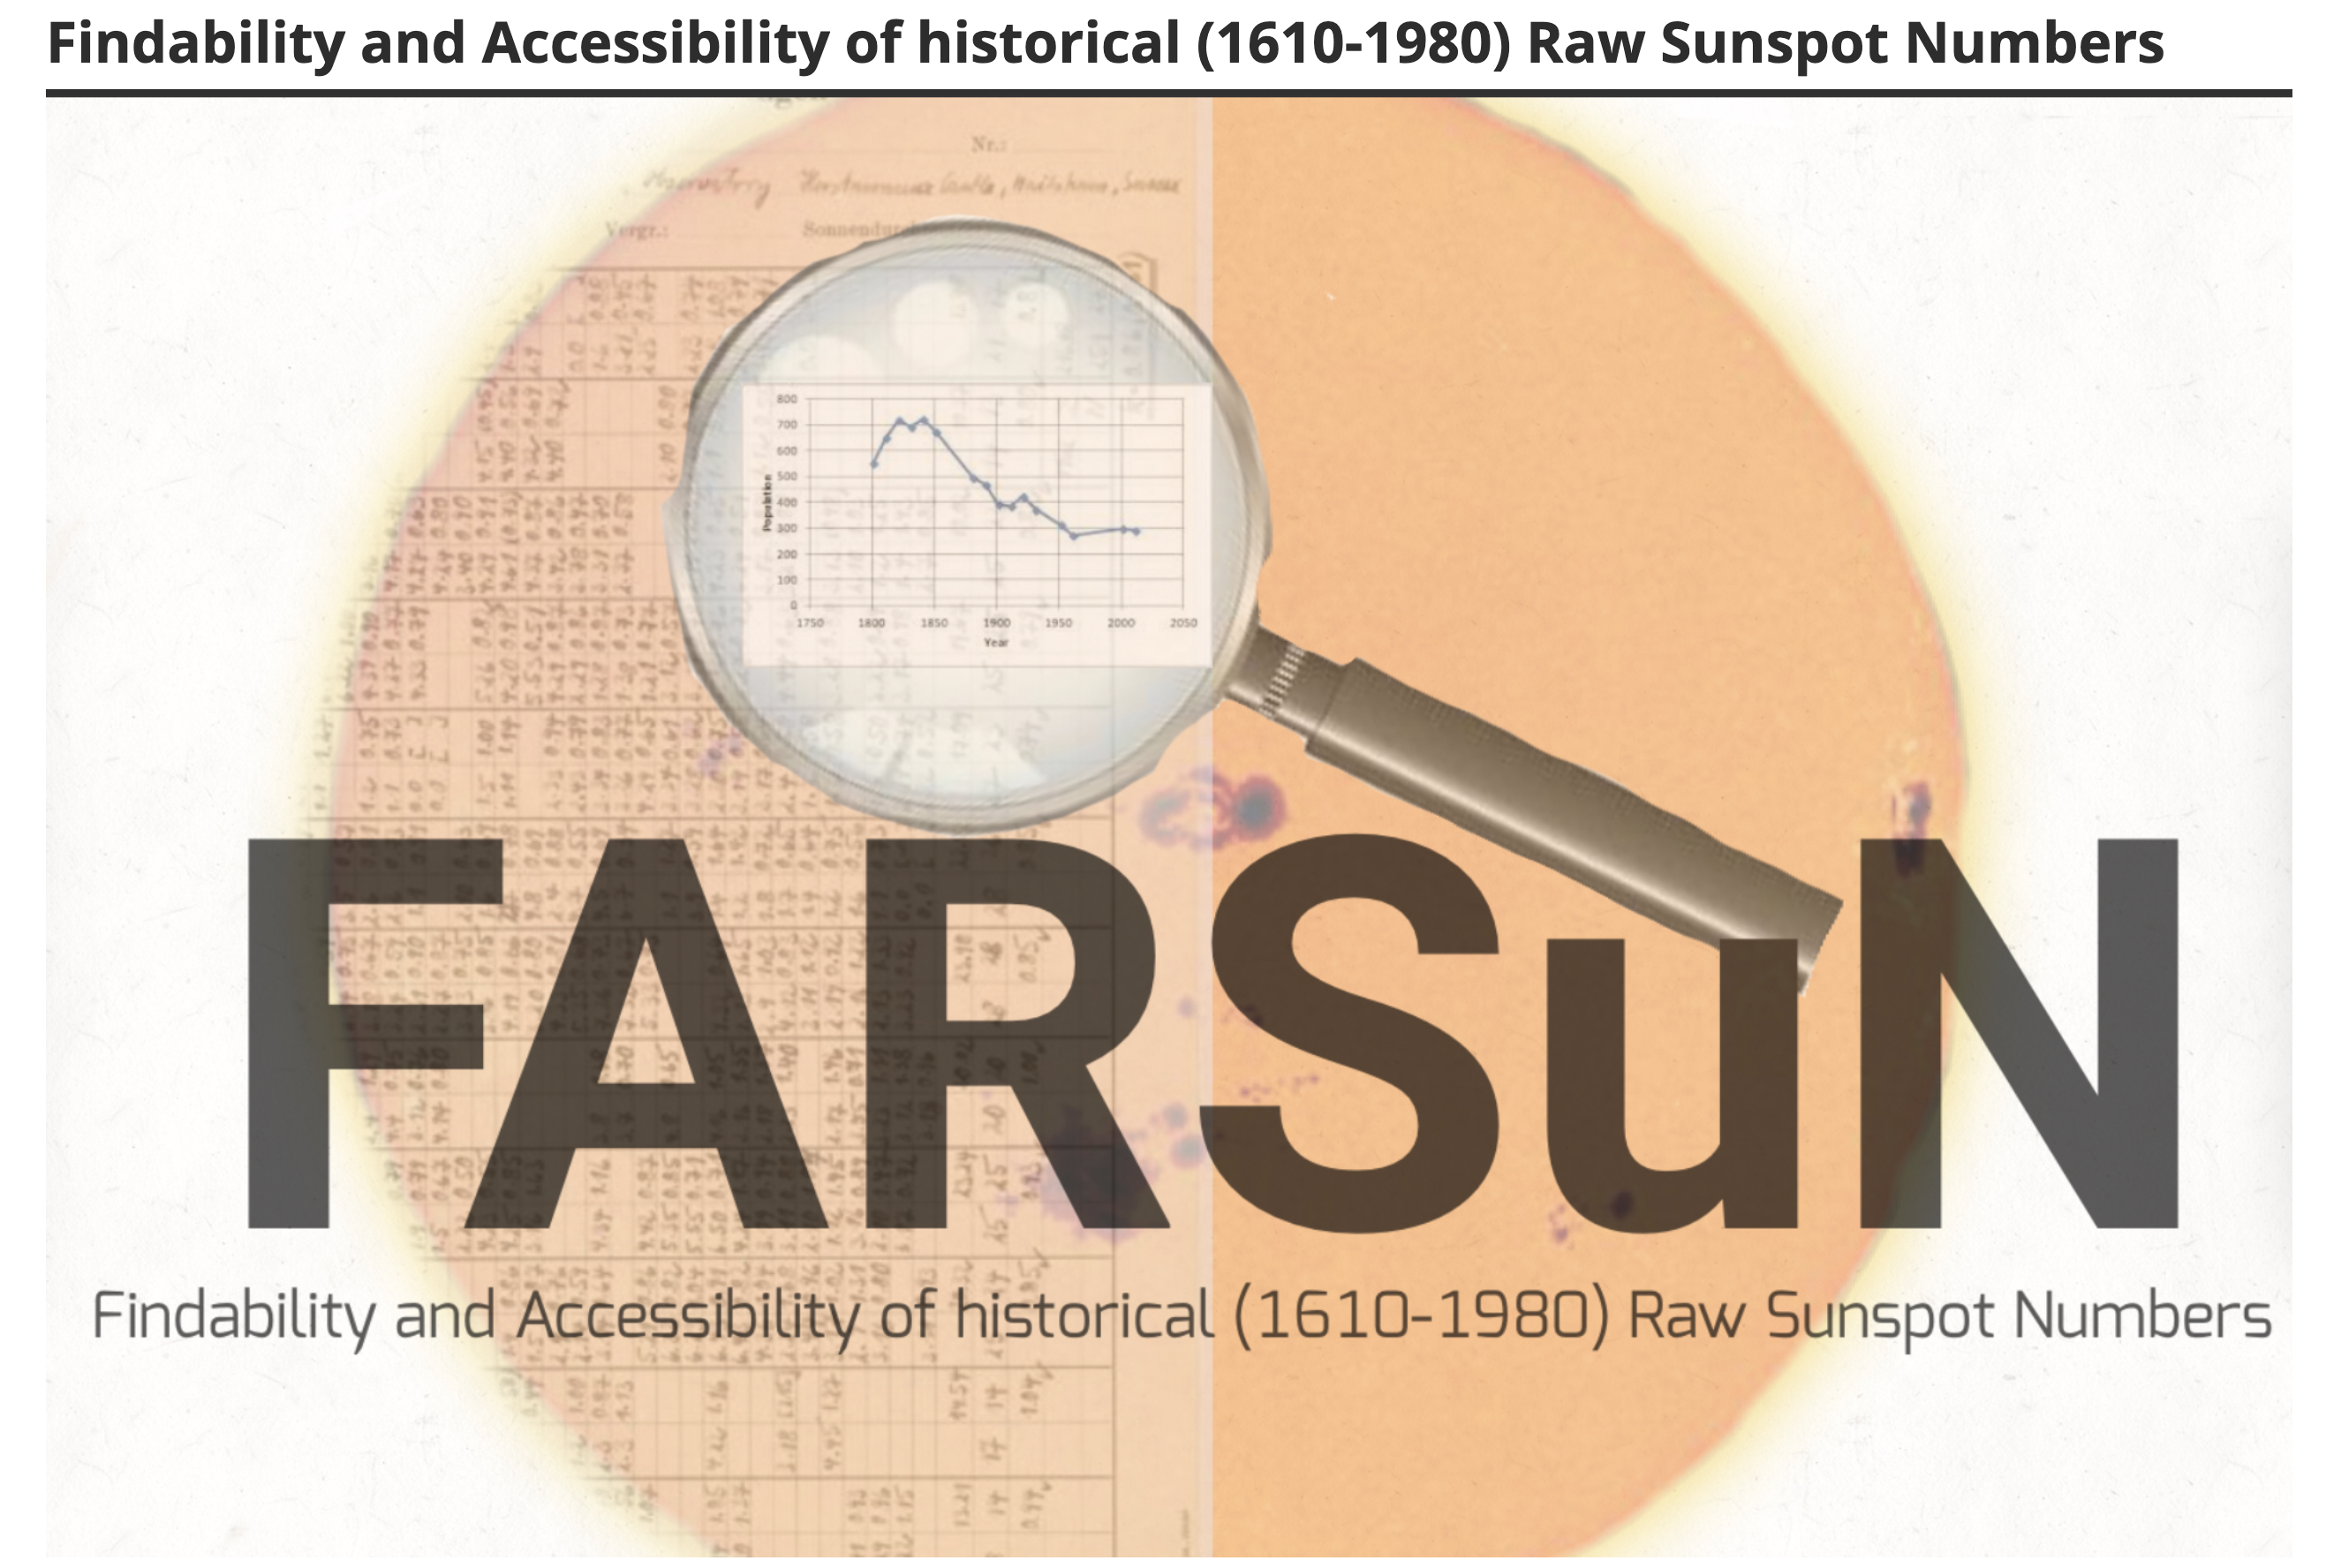
\includegraphics[width=0.45\linewidth]{./figures/ack_.png}
\end{frame}

% --- End ---
\begin{frame}
\centering \Huge Questions?
\end{frame}

\end{document}
